\begin{center}
\textsc{\Large Laboratorio 2}~\\
{\large Vídeo Juegos, Programación, Diseño}~\\
\emph{Cámaras Virtuales}
\end{center}

\section{Pre-Laboratorio}
\todo[inline]{Por hacer.}
\section{Definición}
\begin{wrapfigure}[7]{l}{0.4\linewidth}
\includegraphics[width=\linewidth]{semana2/frustum.eps}
\caption{\emph{Viewing Frustum} de una Camara Virtual donde se muestra el Far y Near Clipping Plane \cite{microsoft_frustum}.}
\label{fig:frustum}
\end{wrapfigure}
En los vídeo juegos se utilizan cámaras virtuales para mostrar un mundo 3D o 2D en algún dispositivo visual. Un sistema virtual de cámaras se encarga de controlar una o mas cámaras en un escenario de juego. Usualmente la cámara en muchos frameworks y bibliotecas para desarrollo de vídeo juegos no es mas que otro objeto en escena \cite{fund_gamedesign}.
\newpage
\section{Conceptos}
Algunos conceptos necesarios para entender el uso de cámaras en la gran mayoría de los frameworks, bibliotecas y motores para el desarrollo de video juegos \cite{unity_camera}.
\subsection{Tipos de Proyección}
\setlength\intextsep{0pt}
\begin{wrapfigure}[7]{r}{0.45\linewidth}
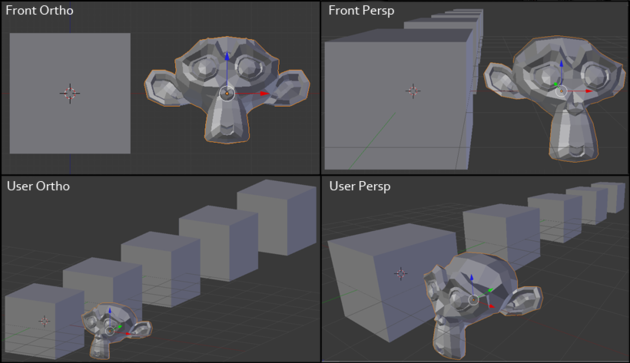
\includegraphics[width=\linewidth]{semana2/projections.png}
\caption{Proyección Ortogonal y Perspectiva.}
\end{wrapfigure}
Existen dos tipos proyección en la mayoría de los frameworks y bibliotecas para el desarrollo de vídeo juegos estos son proyección perspectiva y proyección ortogonal.
\subsubsection{Perspectiva}
Es la forma natural en que el ojo humano percibe una escena, en la proyección perspectiva los objetos distantes se ven mas pequeños que los objetos cercanos dando profundidad a distintos objetos en una escena. Este tipo de proyección es utilizada usualmente en juegos 3D.
\subsubsection{Ortogonal}
En una proyección perspectiva un objeto lejano es mas pequeño que un objeto cercano, en proyección ortogonal se ignora este efecto, eliminando la profundidad de escena. Este tipo de perspectiva es utilizada en muchos juegos 2D.
\subsection{Field Of View (FoV) o Campo de Vista}
Es el ancho del angulo de vista de la cámara, indica la extension de lo puede ver la cámara en cualquier momento, usualmente se mide en ángulos, este angulo puede ser el field of view vertical o el field of view horizontal dependiendo del framework, biblioteca o motor de juego usado (ver \ref{fig:camera}) \cite{feng_fovy}.
\subsection{Clipping Planes o Planos de Clipping}
En computación se manejan términos discretos por lo tanto una cámara no puede ver hacia el infinito, para esto están el far y near clipping planes los cuales indican donde termina el renderizado de escena y donde empieza según la posición de la cámara respectivamente (ver \ref{fig:frustum} y \ref{fig:camera}).
\subsubsection{Near Clipping Plane o Plano de Clipping Cercano}
Es donde empieza a dibujarse los objetos de escena en display, los objetos antes de este punto son ignorados por el motor gráfico.
\subsubsection{Far Clipping Plane o Plano de Clipping Lejano}
Es donde termina de dibujarse los objetos de escena en display, los objetos mas lejanos a este punto son ignorados por el motor gráfico.
\begin{figure}[H]
\centering
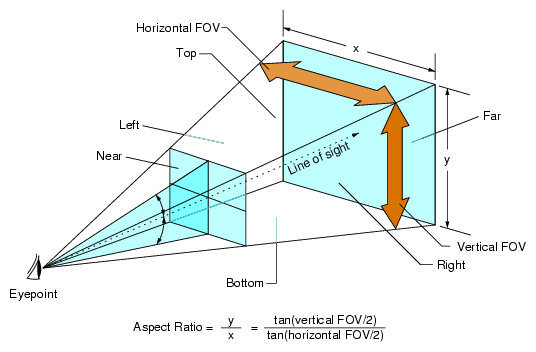
\includegraphics[width=0.9\linewidth]{semana2/camera.png} 
\caption{Parametros de una Camara Virtual}
\label{fig:camera}
\end{figure}
\newpage
\section{Tipos de Sistemas de Cámara en Vídeo Juegos}
Existen principalmente tres tipos de sistemas de cámara en vídeo juegos. En un sistema \emph{fixed} la cámara no cambia sus parámetros originales, un sistema \emph{tracking} sigue algún objeto en juego, y un sistema \emph{interactive} la cámara es parcialmente autónoma y cambia sus parámetros según distintas situaciones. Para implementar distintos sistemas de cámara los desarrolladores de vídeo juegos usan técnicas como programación con restricciones o inteligencia artificial. 
\subsection{Estáticas (\emph{Fixed})}
\begin{wrapfigure}[9]{l}{0.4\linewidth}
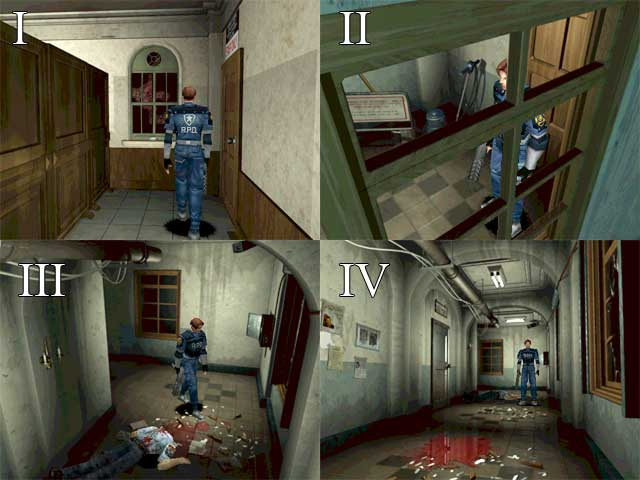
\includegraphics[width=\linewidth]{semana2/resident_evil_camerawork.jpg} 
\caption{Ejemplo de cámaras estáticas en \emph{Resident Evil 2} \cite{fixed_camera}.}
\end{wrapfigure}
En este tipo de cámara las propiedades de la cámara como su posición, orientación y campo visual (\emph{field of view}) son colocadas durante el desarrollo del juego y estas no cambian durante el \emph{gameplay}. Algunos ejemplos de juegos con este tipo de camara son los primeros Resident Evil, y Alone In The Dark, usualmente es utilizada para crear tension \cite{res5_review}\cite{fixed_camera}.
\subsection{Seguidoras (\emph{Tracking})}
Este tipo de cámara sigue a algún objeto en el juego usualmente el personaje principal u otro objeto de considerable importancia. Este sistema presenta varios problemas sobretodo en ambientes tridimensionales y tercera persona donde la cámara podría quedar detrás de una objeto que ocluye totalmente la vista o no deja ver algún objeto de interés al jugador \cite{fund_gamedesign}. Su uso es muy comun en los primeros juegos 3D como \emph{Crash Bandicoot} en tercera persona, los juegos primera persona también utilizan una cámara seguidora, a diferencia de en tercera persona donde la cámara esta detras del personaje en un juego primera persona la cámara esta como visión del personaje principal, en los juegos 2D esta cámara esta presente en todos los juegos tipo side-scroller.
\newpage
\subsection{Interactivas (\emph{Interactive})}
\begin{wrapfigure}[11]{r}{0.4\linewidth}
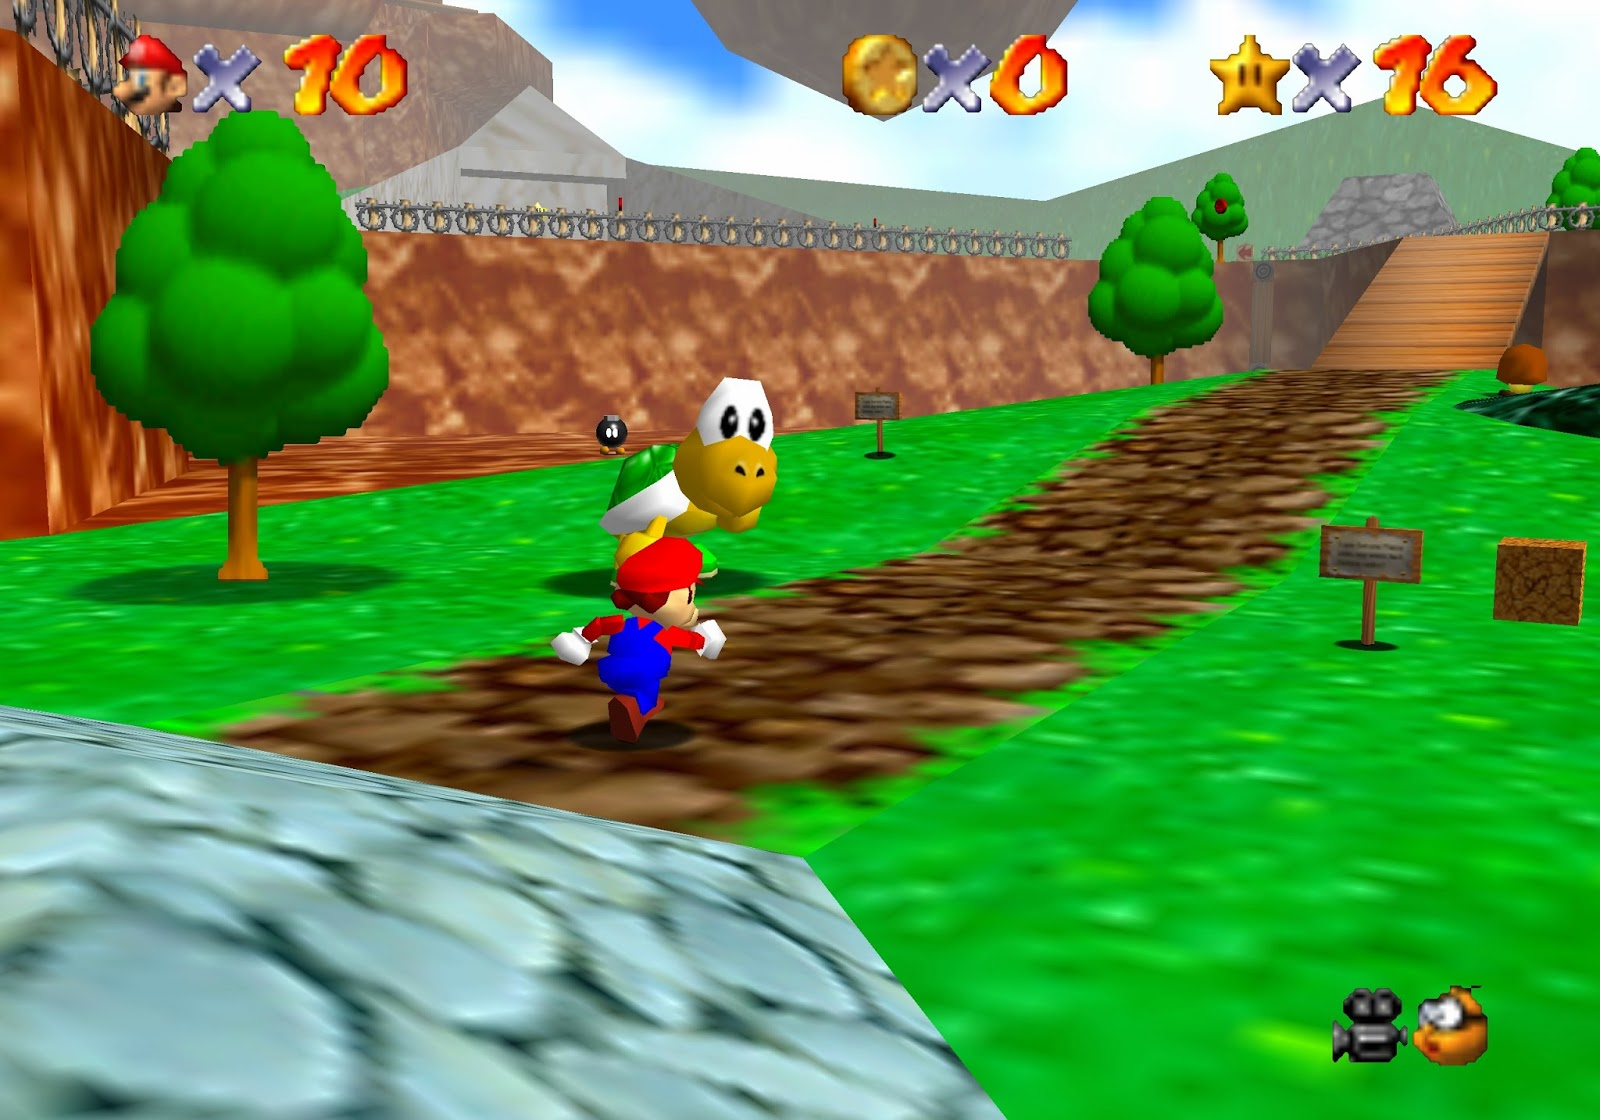
\includegraphics[width=\linewidth]{semana2/supermario64.jpg} 
\caption{En \emph{Super Mario 64} la cámara rota de forma inteligente para mostrar el camino.}
\end{wrapfigure}
Las cámaras interactivas son cámaras que cambian su posición, campo visual u orientación según distintas situaciones, lugares o intereses del juego y sus desarrolladores, usualmente estas cámaras poseen alguna forma de inteligencia artificial. En su mayoría las cámaras interactivas son cámaras tracking mejoradas, estas siguen al personaje como lo hace una cámara tracking pero su posición y orientación puede cambiar si estas se ven obstruidas por algún objeto o cambian sus parámetros para mostrar objetos de interés claramente evitando de esta forma las desventajas principales de una cámara tracking. Algunos ejemplos de juegos con este tipo de camara son \emph{Super Mario 64}, \emph{Super Mario Sunshine}, \emph{The Legend of Zelda: The Wind Waker.}
\section{Actividad}
\todo[inline]{Por hacer.}